%!TEX root = bioPrediction_main.tex

\subsection{Data Preparation}

In this section we describe how we preprocessed the collected data for use in training and testing machine learning models.

\subsubsection{Data Linking}

We linked the collected biometric data and survey responses for each participant. Linking the data is necessary to construct training and test datasets for use in creating and evaluation machine learning models.

Our linking approach is as follows. From the start time of each survey response, we look back one hour for available biometric data. For each minute in that hour-long time window, we check for biometric data to associate with the survey response. For example, if a participant started a survey response at 11:05am, we look for biometric data in the time frame 10:05am to 11:05am. If biometric data is available in the hour-long time window, we consider the survey response to have associated biometric data. Otherwise, we exclude the survey response from our dataset.

Reasons for a survey response to lack associated biometric data include:
\begin{itemize}
\item The participant not wearing the Everion in the hour before before beginning the survey
\item The Everion not recording data in the hour before the participant began the survey (e.g., due to low battery)
\item Biometric data not being uploaded successfully to the server
%\item Compatibility issues between the sensor and the OS tracking the participant's data
%\item Issues accessing the data uploaded by the participants
\end{itemize}

Figure~\ref{surveyBio} illustrates the number of survey responses with associated biometric data for each study participant. 
%This was added to address REviewer 2's concern: Is it correct that the maximum number of responses should have been 112 on the surveys?
The total number of responses per participant is affected by their response rate and by the number days out-of-office (e.g., vacations, holidays, etc.). 
Participant S2 and S12 have particularly low numbers of usable survey responses. In each of these cases, the issue related to biometric data not being uploaded successfully to the server.

\begin{figure}
  \centering
      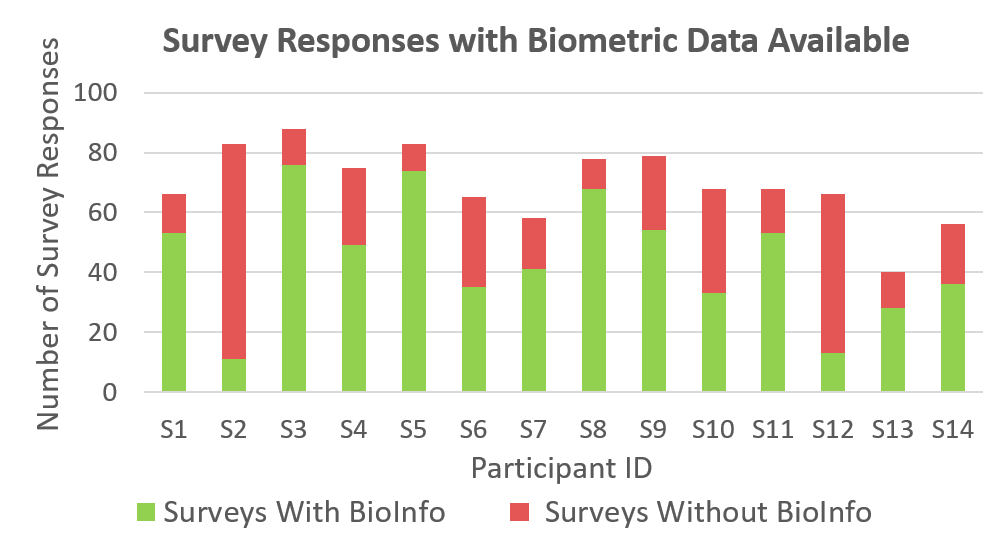
\includegraphics[width=0.5\textwidth]{DuringTheDay.png}
  \caption{The figure shows the biometric data available per each participant. Green sections represent survey responses with biometric
  data available, red sections responses with no biometric data available}
   \label{surveyBio}
   \vspace*{-4mm}
\end{figure}


\subsubsection{Feature Extraction}
We extracted features from the biometric data to provide as input to machine 
learning models. Previous 
studies~ \cite{vorburger05,zuger2015interruptibility} identify time windows as an 
important factor that impacts the prediction accuracy of a classifier. We 
considered many time windows from the literature on biometric 
analysis~\cite{zuger18}, ranging from 10 seconds to 3 hours. Specifically, we 
considered the following time windows: \textit{10sec, 20sec, 30sec, 45sec, 
1min, 2min, 3min, 5min, 7.5min, 10min, 20min, 30min, 45min, 1hour, 2hour, 
3hour}.

From the start time of each survey response, we look back the amount of time 
that corresponds to each time window, and we create features for all of the 
biometric data available in that time window. For example, if a participant 
started a survey response at 11:05am, for the 30min time window, we create 
features using all of the available biometric data from 10:35am to 11:05am. 
For each time window, we calculate 10 statistical measurements from the 
biometric data to create 10 distinct features. Specifically, the 10 
statistical measurements are: mean, standard deviation, variance, median, 
percentile25, percentile75, interquartile range, maximum, minimum, and 
range. Thus, for each survey response, we generate a large number of 
corresponding features based on three factors: biometric measurement, time 
window, and statistical measurement. In addition to these biometric 
features, we also considered the time of day in which the questions were 
asked. These features are created to predict the responses described by the 
ground truth.

\subsubsection{Response Transformations}
Table~\ref{responseDistribution} illustrates the distribution of responses from each participant for each of the three survey questions (listed in Section~\ref{sec:Surveys}). The figure shows that there is a notable imbalance in the distribution of the self-reported responses provided by the participants. Most participants did not use all five points of the five-point Likert scale in their responses, and the distributions tend to skew toward one side or the other, depending on the question. Thus, we binarized the survey data into a two-point scale to give the machine learning models the best possible chance to make useful predictions. The two points in the binary scale represent negative or positive responses for each of the three human aspects of interests (e.g., not stressed or stressed). 

We binarized the survey responses as follows. For each participant, we calculated the median response value for each question. We classified each response below the median as 0 ('negative') and each response above the median as 1 ('positive'). The distribution for the stress question skewed left, so we included the median values in the 'positive' class, while the distributions for focus and awakeness skewed right, so we included those median values in the 'negative' class.

\subsubsection{Oversampling}
Even after binarizing the responses as described in the previous section, we found the distribution of responses was still quite imbalanced for many of our participants. This can be seen in the distribution columns in Table \ref{tab:accuracy}. To combat this, we applied random oversampling to our training sets, which artificially rebalances the dataset by creating randomly replicated data in the minority class. This has been a commonly used technique in previous studies on unbalanced datasets \cite{chawla2004,yap2014}.


\begin{table}
  \centering
      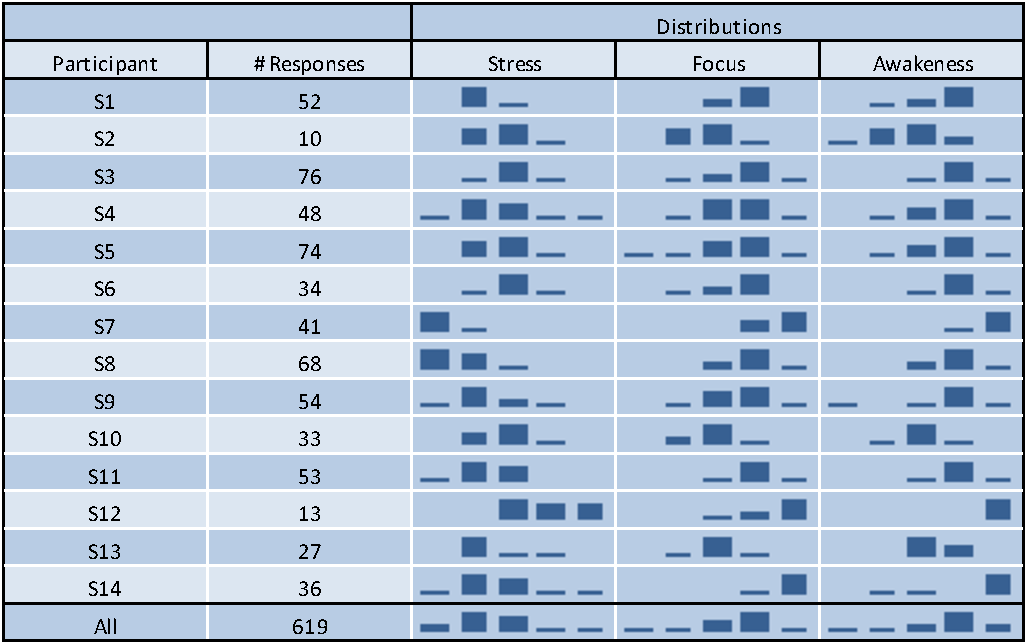
\includegraphics[width=0.5\textwidth]{distributiontable.pdf}
  \caption{The distribution of the responses of each participant to the three questions asked during the day are shown. Each bar in the histograms represent one of the 5 values on the 5-point Likert scale we asked participants to respond with, where the far left side of the histograms are 1/Not at all, and the far right sides are 5/Extremely}
   \label{responseDistribution}
   \vspace*{-2mm}
\end{table}

